\documentclass[10pt]{article}
\usepackage[utf8]{inputenc}
\usepackage[T1]{fontenc}
\usepackage{amsmath}
\usepackage{amsfonts}
\usepackage{amssymb}
\usepackage{mhchem}
\usepackage{stmaryrd}
\usepackage{graphicx}
\usepackage[export]{adjustbox}
\graphicspath{ {./images/} }

\title{BASIC MATH EXPLAINED WITH PRACTICE MATH }

\author{}
\date{}


\begin{document}
\maketitle
Converting (MGD) Million Gallon per Day to (gpd) gallon per day

Converting (MGD) Million Gallon per Day to (gpd) gallon per day

Two methods available to you

$1^{\text {st }}$ Move the decimal to the right 6 places

$2^{\text {nd }}$ Multiply by $1,000,000$

Example: $2.3 \mathrm{MGD}$ to gpd $=2,300000=2,300,000 \mathrm{gpd}$

Or $2.3$ MGD $x 1,000,000=2,300,000 \mathrm{gpd}$

Problems:
$$
\begin{array}{lll}
\text { 1. } & 1.6 \mathrm{MGD}= & \mathrm{gpd} \\
\text { 2. } & 0.04 \mathrm{MGD}= & \mathrm{gpd} \\
\text { 3. } & 0.002 \mathrm{MGD}= & \mathrm{gpd}
\end{array}
$$
Converting $(\mathrm{gpd})$ to (MGD)

Two methods available to you

$1^{\text {st }} \quad$ Move the decimal to the left 6 places

$2^{\text {nd }}$ Divide by $1,000,000$

Example: $1,475,000$ gpd to MGD $=1,475,000=1.475 \mathrm{MGD}$

Or $1,475,000 \mathrm{gpd} \div 1,000,000=1.475 \mathrm{MGD}$

Problems:
$$
\begin{aligned}
& \text { 4. } 100,000 \mathrm{gpd}=\text { MGD } \\
& \text { 5. } 5,300 \mathrm{gpd}=\square \mathrm{MGD} \\
& \text { 6. } 275 \mathrm{gpd} \quad=\text { MGD }
\end{aligned}
$$

\section{Surface Area}
$$
\quad \underline{\text { Squares \& Rectangles }} \quad(\mathrm{A}) \mathrm{ft}^{2}=(\mathrm{L} \times \mathrm{W}) \quad \text { Area } \mathrm{ft}^{2}=(\text { Length } \mathrm{x} \text { Width })
$$

\section{Example:}
A surface dimensions are $35 \mathrm{ft}$. long by $15 \mathrm{ft}$. wide. What is the Area $\mathrm{ft}^{2}$ ?

Area $\mathrm{ft}^{2}=($ Length $35 \mathrm{ft}$. x Width $15 \mathrm{ft} .) \quad$ Area $=(35 \mathrm{ft} . \mathrm{x} 15 \mathrm{ft}) \quad$ Area $=525 \mathrm{ft}^{2}$

\section{Problems:}
\begin{enumerate}
  \setcounter{enumi}{7}
  \item $\mathrm{L}=40 \mathrm{ft} . \mathrm{W}=20 \mathrm{ft}$. Surface Area $=$

  \item $\mathrm{L}=15 \mathrm{ft}$. $\mathrm{W}=5 \mathrm{ft}$. Surface Area $=$ $\mathrm{ft}^{2}$ $\mathrm{ft}^{2}$

\end{enumerate}
\section{Volume}
Squares \& Rectangles

Third dimension $=$ Height or Depth

(V) $\mathrm{ft}^{3}=(\mathrm{L} \times \mathrm{W} \times$ Third dimension $)$

\section{Example:}
A Sedimentation basin dimensions are $40 \mathrm{ft}$. long $20 \mathrm{ft}$. wide and $14 \mathrm{ft}$. deep.

What is the Volume $\mathrm{ft}^{3}$ ?

Volume $\mathrm{ft}^{3}=($ Length $40 \mathrm{ft}$. $x$ Width $20 \mathrm{ft}$. x Depth $14 \mathrm{ft}$. $)$
$$
=(40 \mathrm{ft} \text {. } 20 \mathrm{ft} \text {. } 14 \mathrm{ft} \text {. })
$$
$$
=11,200 \mathrm{ft}^{3}
$$

\section{Problems:}
$$
\begin{aligned}
& \text { 9. } \mathrm{L}=40 \mathrm{ft} . \quad \mathrm{W}=20 \mathrm{ft} . \mathrm{D}=10 \mathrm{ft} . \quad \text { Volume }=\mathrm{ft}^{3} \\
& \text { 10. } \mathrm{L}=15 \mathrm{ft} . \quad \mathrm{W}=5 \mathrm{ft} . \quad \mathrm{D}=8 \mathrm{ft} . \quad \text { Volume }=\stackrel{\mathrm{ft}^{3}}{ }
\end{aligned}
$$

\section{Surface Area}
Cylinders (Round Tanks, Pipe, Clarifiers, etc)

Surface Area $\mathrm{ft}^{2}=\pi \mathrm{r}^{2}=\pi \mathrm{x}$ radius $\mathrm{ft}$. $\mathrm{x}$ radius $\mathrm{ft}$.
$$
\pi=3.14 \quad r=\text { Radius }=1 / 2 \text { Diameter }
$$
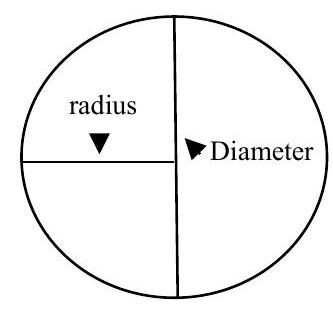
\includegraphics[max width=\textwidth]{2022_09_16_0c6b804a9b26a8df4e8fg-02}

Example: A Clarifier has a diameter of $40 \mathrm{ft}$. What is the Surface Area $\mathrm{ft}^{2}$ ?

Surface Area $=\pi \times 20 \mathrm{ft}$. $\times 20 \mathrm{ft}$. $=3.14 \times 20 \mathrm{ft}$. $20 \mathrm{ft} .=1,256 \mathrm{ft}^{2}$

\section{Problems:}
$$
\begin{aligned}
& \text { 11. } \quad \text { Diameter }=30 \mathrm{ft} \text {. } \\
& \text { Surface Area }= \\
& \text { 12. Diameter }=75 \mathrm{ft} \text {. } \\
& \text { Surface Area }= \\
& \mathrm{ft}^{2} \\
& \mathrm{ft}^{2}
\end{aligned}
$$

\section{Volume}
Cylinders (Round Tanks, Pipe, Clarifiers, etc)

Volume $\mathrm{ft}^{3}=\pi \mathrm{r}^{2} \mathrm{x}$ third dimension
$$
=\pi \mathrm{x} \text { radius } \mathrm{ft} \text {. } \mathrm{x} \text { radius } \mathrm{ft} \text {. } \mathrm{x} \text { third dimension } \mathrm{ft} \text {. }
$$
$\pi=3.14 \quad r=$ Radius $=1 / 2$ Diameter $\quad$ Third dimension $=$ Height or Depth

\section{Example:}
A Clarifier has a diameter of $40 \mathrm{ft}$. and a depth of $14 \mathrm{ft}$. What is the Surface Area $\mathrm{ft}^{3}$ ?

Surface Area $=\pi \times 20 \mathrm{ft}$. $20 \mathrm{ft}$. $14 \mathrm{ft}$.
$$
=3.14 \times 20 \mathrm{ft} . \mathrm{x} 20 \mathrm{ft} . \mathrm{x} 14 \mathrm{ft} .=17,584 \mathrm{ft}^{3}
$$

\section{Problems:}
\begin{enumerate}
  \setcounter{enumi}{13}
  \item Diameter $=30 \mathrm{ft} . \quad$ Depth $=10 \mathrm{ft} . \quad$ Volume $=\quad \mathrm{ft}^{3}$

  \item Diameter $=75 \mathrm{ft} . \quad$ Depth $=14 \mathrm{ft} . \quad$ Volume $=\quad \mathrm{ft}^{3}$

\end{enumerate}
\section{Volume $\mathrm{ft}^{3}$ to Volume gallons}
Volume $\mathrm{ft}^{3} \times \mathrm{gal} / \mathrm{ft}^{3} \quad$ Gallons $=$ Volume $\mathrm{ft}^{3} \times 7.48 \mathrm{gal} / \mathrm{ft}^{3}$

\section{Example:}
Volume of a tank $=17,584 \mathrm{ft}^{3}$ How many gallons can this tank hold?
$$
\text { Gallons }=\left(17,584 \mathrm{ft}^{3} \times 7.48 \mathrm{gal} / \mathrm{ft}^{3}\right) \quad \text { Gallons }=131,528.32 \text { or } 0.13 \mathrm{MG}
$$

\section{Problems:}
$$
\begin{aligned}
& \text { 15. } \quad 495 \mathrm{ft}^{3} \\
& \text { gal. = } \\
& \text { MG } \\
& \text { 16. } 1,295 \mathrm{ft}^{3} \\
& \text { gal. = } \\
& \text { MG }
\end{aligned}
$$

\section{Volume gallons to (lbs) Pounds 
 $\mathrm{lbs}=$ gallons x $8.34 \mathrm{lbs} / \mathrm{gal}$}
\section{Example:}
131,528 gallons to $\mathrm{lbs}=131,528 \mathrm{gal}$ x $8.34 \mathrm{lbs} / \mathrm{gal}=1,096,943.52 \mathrm{lbs}$. or $1.1 \mathrm{Mlbs}$

\section{Problems:}
\begin{enumerate}
  \setcounter{enumi}{17}
  \item 595 gallons $=$ lbs. $=$ Mlbs

  \item 1,397 gallons $=$ lbs. $=$ Mlbs

\end{enumerate}
\section{Circumference}
Circumference of a circle $=\pi \mathrm{x}$ diameter $\mathrm{ft}$.
$$
=3.14 \mathrm{x} \text { diameter } \mathrm{ft} \text {. }
$$

\section{Example:}
The Diameter $=40 \mathrm{ft}$. What is the Circumference $\mathrm{ft}$.

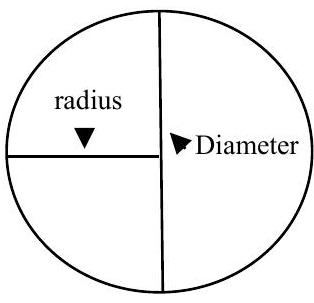
\includegraphics[max width=\textwidth]{2022_09_16_0c6b804a9b26a8df4e8fg-03}
$$
\begin{aligned}
\text { Circumference ft. } &=\pi \times 40 \\
&=3.14 \times 40 \\
&=125.6 \mathrm{ft} .
\end{aligned}
$$

\section{Problems:}
\begin{enumerate}
  \setcounter{enumi}{19}
  \item Diameter $=30 \mathrm{ft} . \quad=$ Circumference $\mathrm{ft}$.

  \item Diameter $=75 \mathrm{ft}$. $=$ Circumference $\mathrm{ft}$.

\end{enumerate}
\section{Convert psi to ft.}
$2.31 \mathrm{ft}$ of head $=1 \mathrm{psi} \quad 1 \mathrm{ft}$ of head $=0.433 \mathrm{psi}$

Example: $\quad 30 \mathrm{psi}=$ how many $\mathrm{ft}$ of head

or
$$
\begin{array}{ll}
\mathrm{ft} .=30 \mathrm{x} 2.31 \mathrm{ft} . / \mathrm{psi} & \mathrm{ft}=69.3 \mathrm{ft} . \\
\mathrm{ft} .=30 \div 0.433 \mathrm{psi} / \mathrm{ft} . & \mathrm{ft} .=69.3 \mathrm{ft} .
\end{array}
$$
Problems:
$$
\begin{aligned}
& \text { 21. } \mathrm{psi}=53 \quad \mathrm{~L} \quad \mathrm{ft} \text {. } \\
& \text { 22. } \mathrm{psi}=125=\mathrm{ft} \text {. }
\end{aligned}
$$

\section{Convert ft. to psi}
Example: $100 \mathrm{ft}$. of water is in the tower. What would the psi gage read?
$$
\begin{array}{ll}
\text { psi } & =100 \mathrm{ft} . \div 2.31 \mathrm{ft} . / \mathrm{psi} \\
\text { or } \quad & \mathrm{psi}=43.3 \\
\mathrm{psi} & =100 \mathrm{ft} . \times 0.433 \mathrm{psi} / \mathrm{ft} . \\
\mathrm{psi} & =43.3
\end{array}
$$

\section{Problems:}
$$
\begin{aligned}
& \text { 43. } \mathrm{ft} .=125 \quad=\quad \text { psi } \\
& \text { 44. } \mathrm{ft} .=55 \quad=\ldots \mathrm{psi}
\end{aligned}
$$

\section{Review}
\begin{itemize}
  \item $\underline{\text { Area of square or rectangle }}=(\mathrm{L} \times W)=\mathbf{f t}^{2}$

  \item $\quad$ Area of a circle $=\left({ }^{66} \pi^{99} 3.14 \times \mathbf{r}^{2}\right)=\mathrm{ft}^{2}$

  \item Volume of sq or rectangle $=(\mathrm{L} \times \mathbf{W} \times \mathbf{H})=\mathbf{f t}^{3}$

  \item Volume of cylinder $=\left({ }^{66} \pi^{99} 3.14 \times \mathbf{r}^{2} \times H\right)=\mathrm{ft}^{3}$

  \item $\underline{\text { Volume gal }}=\left(f^{3} \times 7.48 \mathrm{gal} / \mathrm{ft}^{3}\right)=$ gallons

  \item Diameter to Circumference $=\pi \times$ diameter

  \item $\quad \underline{l b s}=(g a l l o n s ~ \times 8.34 ~ l b s / g a l)$

  \item From Volume to lbs

  \item $(\mathrm{L} \times \mathrm{W} \times \mathrm{H})\left(7.48 \mathrm{gal} / \mathrm{ft}^{3}\right)(8.34 \mathrm{lbs} / \mathrm{gal})=\mathrm{lbs}$

  \item $\left(\pi 3.14 \times \mathbf{r}^{2} \times \mathrm{H}\right)\left(7.48 \mathrm{gal} / \mathrm{ft}^{3}\right)(8.34 \mathrm{lbs} / \mathrm{gal})=\mathrm{lbs}$

\end{itemize}
\section{Remember radius must be in FEET to work for the purpose of the equations listed above}
\begin{itemize}
  \item Flow MGD $\times 8.34=$ Mlbs

  \item Volume MG $\times 8.34=$ Mlbs

  \item Volume gal $\times 8.34=\mathrm{lbs}$

\end{itemize}
\section{Volume Gallons:}
\section{Example:}
You have just laid a section of pipe which is 18 " in diameter and 2,850 ft. long. How many gallons does this section of pipe hold?

Formula $\left(\pi \mathrm{r}^{2} \mathrm{ft}\right.$. x length $\mathrm{ft}$. $\left.7.48 \mathrm{gal} / \mathrm{ft}^{3}\right)$

$1^{\text {st }}$. you have to convert the diameter from inches to feet.

$18 " \div 12 " / \mathrm{ft}$. $=1.5 \mathrm{ft}$. DIAMETER Be sure to remember this is still DIAMETER

$2^{\text {nd }}$ now you have to divide the DIAMETER by 2 to get to radius

$1.5 \mathrm{ft} . \div 2=0.75 \mathrm{ft}$. RADIUS

$3^{\text {rd }}$ work the formula

Formula $\left(\pi r^{2} ft^2 \right.\times length \mathrm{ft}\times \left.7.48 \mathrm{gal} / \mathrm{ft}^{3}\right)$

$(3.14 \times 0.75 \mathrm{ft} \times 0.75 \mathrm{ft}\times 2,850 \mathrm{ft} \times 7.48 \mathrm{gal} / \mathrm{ft} 3)=$

$37,652.9175$ gallons ROUND TO 37,653 gallons

\section{Problems:}
\begin{enumerate}
  \setcounter{enumi}{25}
  \item You have just laid a section of pipe which is 6 " in diameter and 1,200 ft. long. How many gallons does this section of pipe hold?

  \item Your crew just finished laying a 18" diameter pipe 1,750 feet. How many gallons would that section of pipe hold?

\end{enumerate}
\section{Volume to drainage time:}
\section{Example:}
It is time to drain your sedimentation basin for cleaning, the dimensions of the tank is 85 feet long, 40 feet wide and 15 feet deep. Using a pump that has a pumping rate of 185 gpm figure how many hours would this process take.

$1^{\text {st }}$ you have to figure how many gallons is in the tank.

Formula Gallons $=\left(\right.$ Length $\mathrm{ft}$. $\mathrm{x}$ Width $\mathrm{ft}$. $\mathrm{x}$ Depth $\left.\mathrm{ft} . \mathrm{x} 7.48 \mathrm{gal} / \mathrm{ft}^{3}{ }^{3}\right)$

Gallons $\left.=\left(85 \text { feet long x } 40 \mathrm{ft} \text {. wide x } 15 \mathrm{ft} \text {. } 7.48 \mathrm{gal} / \mathrm{ft} .^{3}\right)^{2}\right)$

Gallons $=381,480$

$2^{\text {nd }}$ you need to divide the number of gallons by the pumping rate of the motor.

In this case the motor is listed as $185 \mathrm{gpm}$

Minutes $=(381,480$ gallons $\div 185 \mathrm{gpm})=2,062.05$ minutes

$3^{\text {rd }}$ you still have at least one more step to convert minutes to hours

Hours $=(2,062.05 \div 60)=34.3675$ hours rounded to $34.37$ hours

\section{NOTE THE ANSWERS MAY BE IN HOURS AND MINUTES SO YOU HAVE ANOTHER STEP}
34.37 HOURS IS NOT 34 HOURS 37 MINUTES YOU MUST MULTIPLE 60 MINUTES/HOUR BY $0.37$ HOURS TO GET MINUTES Minutes $=(60 \times 0.37)=22.2$ minutes rounded to 22 minutes Makes your answer to be 34 HOURS and 22 MINUTES

\section{Problems:}
\begin{enumerate}
  \setcounter{enumi}{27}
  \item It is time to drain your sedimentation basin for cleaning, the dimensions of the tank is 120 feet long, 50 feet wide and 18 feet deep. Using a pump that has a pumping rate of 275 gpm figure how many hours this process would take.

  \item It is time to drain your sedimentation basin for cleaning, the dimensions of the tank is 60 feet long, 30 feet wide and 14 feet deep. Using a pump that has a pumping rate of $185 \mathrm{gpm}$ figure how hours this process would take. Dosage Questions using $100 \%$ Chlorine Gas, Alum or any $100 \%$ Available Chemical:\\

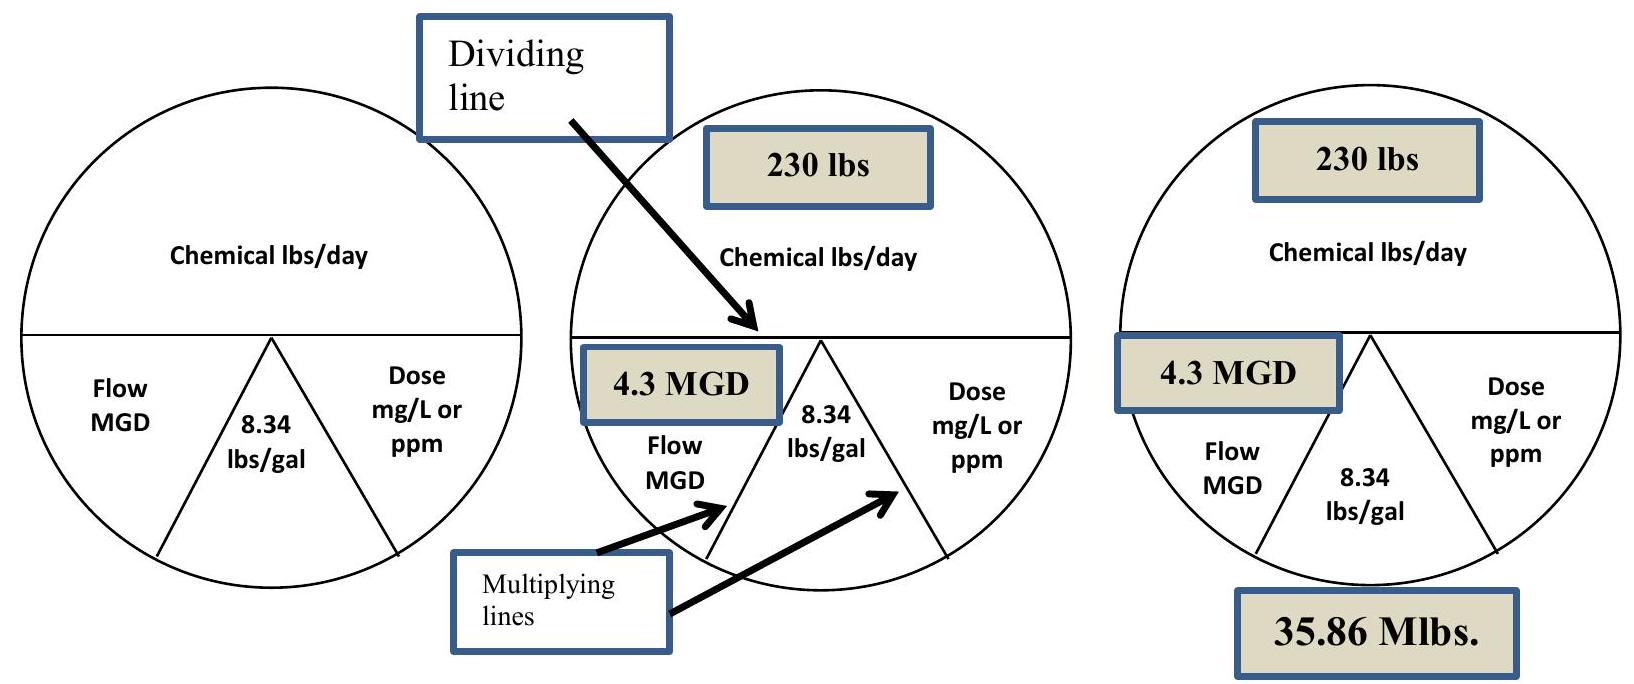
\includegraphics[max width=\textwidth]{2022_09_16_0c6b804a9b26a8df4e8fg-07}

\end{enumerate}
\section{Example:}
The city water usage demand is $4.3$ MGD from the water plant. The water plant is feeding $230 \mathrm{lbs}$./day of chlorine gas. What is the dose in $\mathrm{mg} / \mathrm{L}$ ?

$1^{\text {st }}$ Place the numbers where they belong on the pie as shown above.

$2^{\text {nd }}$ You need to multiply the bottom numbers on the bottom of the pie.

4.3 MGD x $8.34 \mathrm{lbs} / \mathrm{gal}=\mathbf{3 5 . 8 6}$ Mlbs now write this below your pie.

$3^{\text {rd }}$ To understand the way a pie works you need only remember that the half that needs no other information is divided by the half that is needing information to be full.

The top half needed only one piece of information to be full, which has already been given. The bottom half needed three pieces of information to be full but was only given two. So the top half is divided by the bottom half
$$
230 \text { lbs. } \div 35.86 \text { Mlbs. }=\mathbf{6 . 4 1} \mathbf{~ m g} / \mathbf{L} \text { DOSE }
$$
Now to work the same problem using the formula given to us to use by DEQ.
$$
\begin{gathered}
\text { Dose } m g / L=\frac{\text { Chemical, } l b s .}{M l b s} \\
\text { Dose, } m g / L=\frac{230 \text { Chemical,lbs. }}{(4.3 \text { Flow,MGD } x 8.34 l b s / g a l)}=\frac{230 l b s}{35.86 \mathbf{M l b s}}=\mathbf{6 . 4 1} \mathbf{~ m g} / \mathbf{L ~ D O S E}
\end{gathered}
$$

\section{Problems:}
\begin{enumerate}
  \setcounter{enumi}{29}
  \item The city water usage demand is $2.8$ MGD from the water plant. The water plant is feeding $35 \mathrm{lbs} . /$ day of chlorine gas. What is the dose in $\mathrm{mg} / \mathrm{L}$ ?

  \item The city water usage demand is $10.7$ MGD from the water plant. The water plant is feeding $161 \mathrm{lbs}$./day of chlorine gas. What is the dose in $\mathrm{mg} / \mathrm{L}$ ?

  \item The city water usage demand is $1.2 \mathrm{MGD}$ from the water plant. The water plant is feeding $15 \mathrm{lbs}$./day of the coagulant ALUM. What is the dose in $\mathrm{mg} / \mathrm{L}$ ?

  \item The city water usage demand is $5.9 \mathrm{MGD}$ from the water plant. The water plant is feeding $64 \mathrm{lbs}$./day of the coagulant ALUM. What is the dose in $\mathrm{mg} / \mathrm{L}$ ?

\end{enumerate}
\section{Dosage Questions using 65\% or $0.65$ Calcium Hypochlorite or HTH:}
Can also be used for any product with less than $100 \%$ available chemical

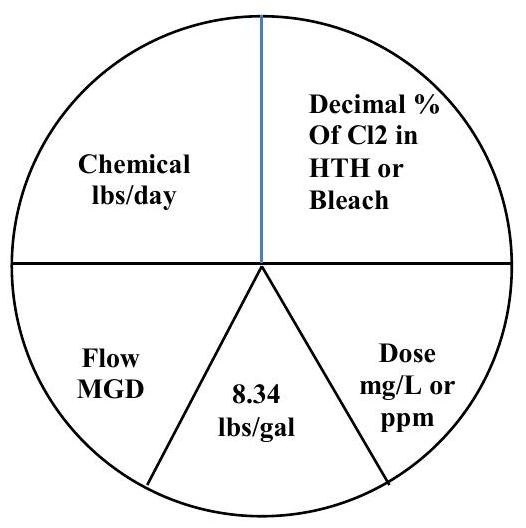
\includegraphics[max width=\textwidth]{2022_09_16_0c6b804a9b26a8df4e8fg-08}

\section{Example:}
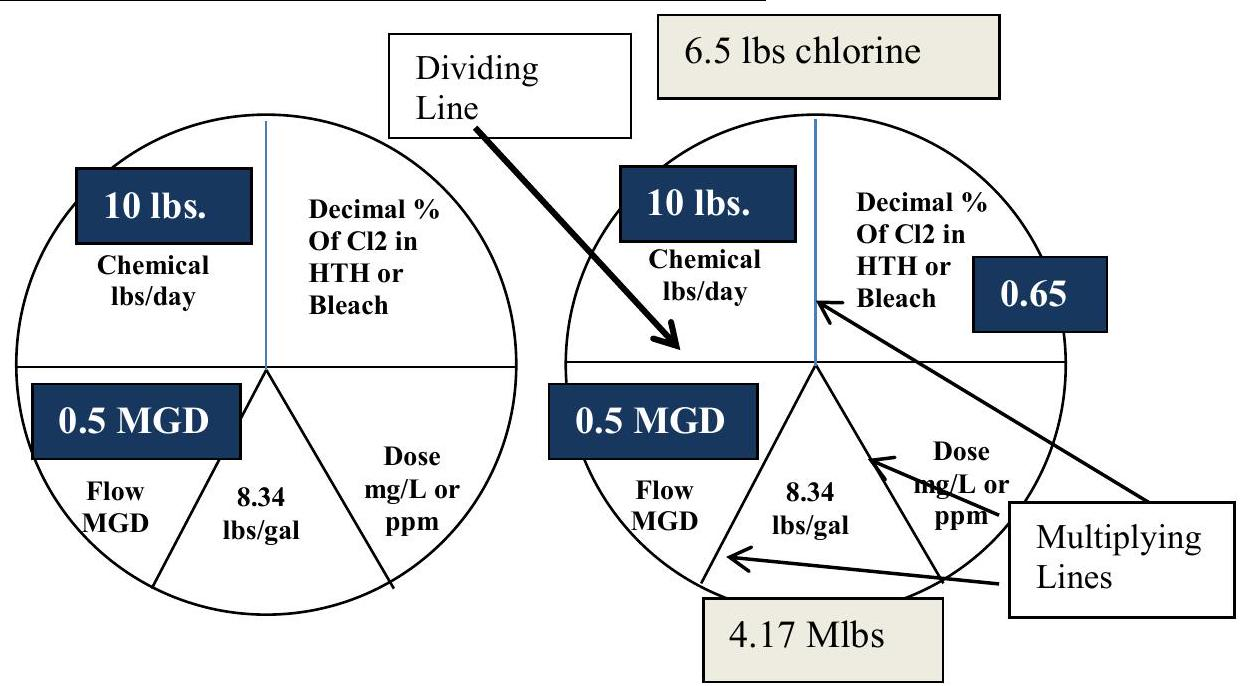
\includegraphics[max width=\textwidth]{2022_09_16_0c6b804a9b26a8df4e8fg-08(1)}

The well is pumping $0.5 \mathrm{MGD}$. You are feeding $10 \mathrm{lbs} /$ day of $\mathrm{HTH} /$ day. What is your dose $\mathrm{mg} / \mathrm{L}$ ?

$1^{\text {st }}$ Place the numbers where they belong on the pie as shown above

$2^{\text {nd }}$ You need to realize that $10 \mathrm{lbs}$ of $\mathrm{HTH}$ is not $10 \mathrm{lbs}$ of chlorine and we are only interested in the amount of chlorine that is being fed.

$\mathrm{HTH}$ is only $65 \%$ chlorine which in decimal form is $0.65$

So if you multiply the top half of the pie you will find out how many lbs. of Chlorine is available.

$10 \mathrm{lbs}$ of HTH x $0.65=6.5 \mathrm{lbs}$ of Chlorine. Write that on the top of your pie.

$3^{\text {rd }}$ You need multiply the numbers on the bottom half of the pie.

$0.5 \mathrm{MGD} \times 8.34 \mathrm{lbs} / \mathrm{gal}=4.17 \mathrm{Mlbs}$. Write that on the bottom of your pie. Remember the way a pie works you need only remember that the half that needs no other information is divided by the half that is needing information to be full.

$4^{\text {th }}$ In this case the top half has all the information it needs and the bottom half is still needing the Dose $\mathrm{mg} / \mathrm{L}$ figured out so the top number is divided by the bottom number.

\section{$6.5 \mathrm{lbs} /$ day chlorine $\div 4.17 \mathrm{Mlbs}=\mathbf{1 . 5 6} \mathbf{~ m g} / \mathbf{L}$ dose}
Now work the same problem using the formula given to us to use by DEQ. However, you notice the formula given is only for $100 \%$ chlorine, you have to add in the difference in $\%$.
$$
\begin{gathered}
\text { Dose, } m g / L=\frac{\text { Chemical, lbs. }}{\text { Flow, Mlbs. }} \\
\text { Dose, } m g / L=\frac{\text { Chemical, lbs. } x 0.65}{\text { Flow, Mlbs. }} \\
\text { Dose }, m g / L=\frac{\text { Chemical, } l b s . x 0.65}{(\text { Flow, } M G D \times 8.34 \mathrm{lbs} / \mathrm{gal})}
\end{gathered}
$$
Dose,$m g / L=\frac{10 \text { Chemical, }, \text { bs. } x 0.65}{(0.5 \mathrm{Flow}, M G D \times 8.34 \mathrm{lbs} / \mathrm{gal})}=\frac{6.5 \mathrm{lbs}}{4.17 \mathrm{Mlbs}}=\mathbf{1 . 5 6} \mathbf{~ m g} / \mathbf{L}$ dose

\section{Problems:}
\begin{enumerate}
  \setcounter{enumi}{33}
  \item The city water usage demand is $2.8 \mathrm{MGD}$ from the water plant. The water plant is feeding $27 \mathrm{lbs} . /$ day of $\mathrm{HTH}$. What is the dose in $\mathrm{mg} / \mathrm{L}$ ?

  \item The city water usage demand is $250 \mathrm{gpm}$ from the water plant. The water plant is feeding $7.5 \mathrm{lbs}$./day of $\mathrm{HTH}$. What is the dose in $\mathrm{mg} / \mathrm{L}$ ? Lbs./day Questions using $100 \%$ Chlorine Gas, Alum or any $100 \%$ Available Chemical:\\

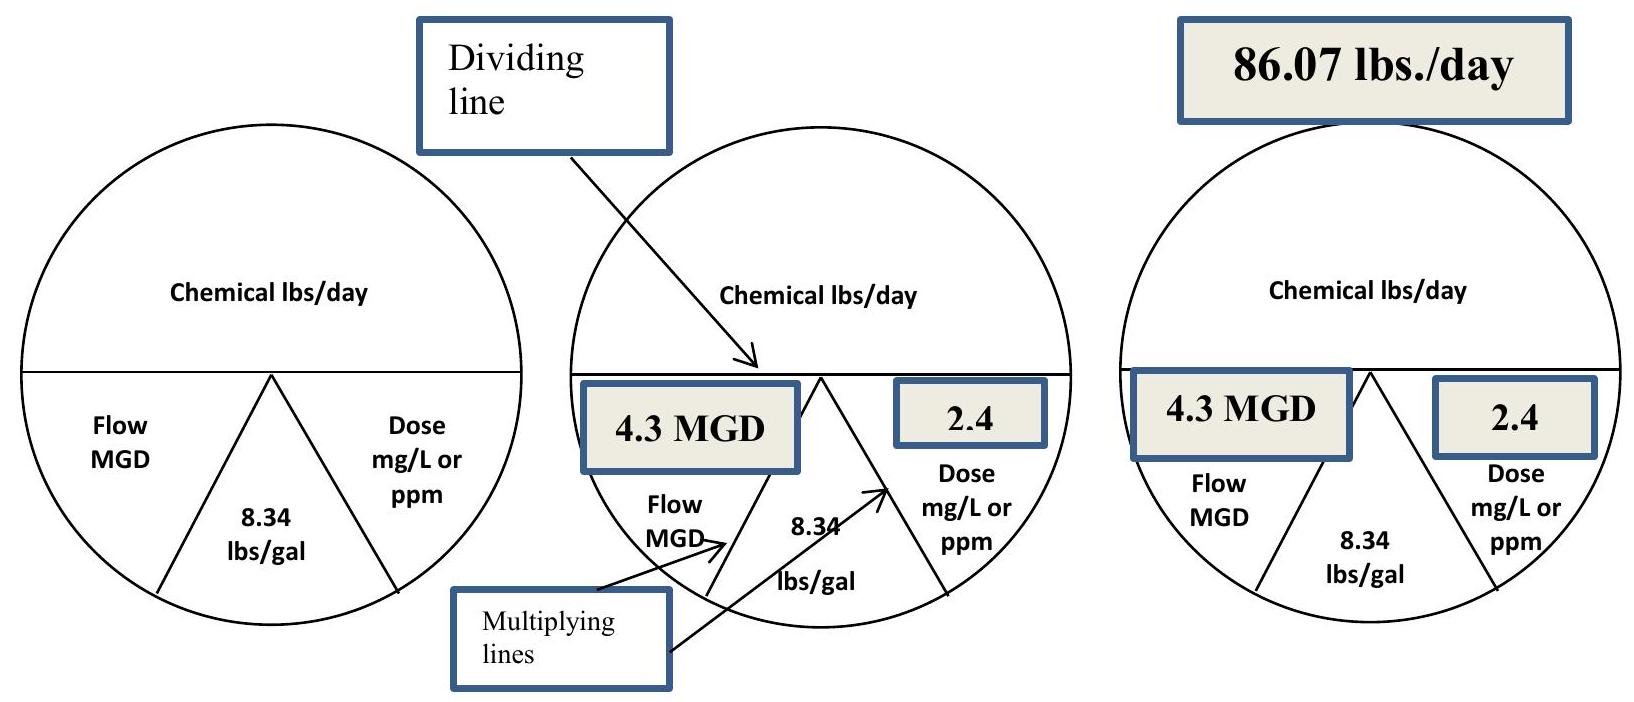
\includegraphics[max width=\textwidth]{2022_09_16_0c6b804a9b26a8df4e8fg-10}

\end{enumerate}
\section{Example:}
The city water usage demand is $4.3 \mathrm{MGD}$ from the water plant. The water plant needs to dose with a $2.4 \mathrm{mg} / \mathrm{L}$ of chlorine gas. How many lbs./day of chlorine gas would you need to feed?

$1^{\text {st }}$ Place the numbers where they belong on the pie as shown above.

$2^{\text {nd }}$ You need to multiply the bottom numbers on the bottom of the pie.
$$
\begin{array}{r}
4.3 \mathrm{MGD} \times 8.34 \mathrm{lbs} / \mathrm{gal} \times 2.4 \mathrm{mg} / \mathrm{L}=\mathbf{8 6 . 0 7} \mathrm{lbs} / \text { day } \\
\text { now write this in the upper section of the pie. }
\end{array}
$$
Since the bottom half of the pie had all the information it needed you can see that all you had to do is multiply those numbers to figure out how many lbs/day of $100 \%$ Chlorine was needed

Now to work the same problem using the formula given to us to use by DEQ.

Chemical Feed, lbs $=($ Dose, mg/L $x$ Flow, Mlbs $)$

Formula expanded:
$$
\begin{gathered}
\text { Chemical Feed, } l b s=(\text { Dose }, \mathrm{mg} / \mathrm{L} \times 8.34 \mathrm{lbs} / \mathrm{gal} x \text { Flow, } M G D) \\
\text { Chemical Feed }, \mathrm{lbs}=(2.4 \mathrm{mg} / \mathrm{L} \times 8.34 \mathrm{lbs} / \mathrm{gal} \times 4.3 \mathrm{MGD})
\end{gathered}
$$
Chemical Feed,lbs $=86.07$

\section{Problems:}
\begin{enumerate}
  \setcounter{enumi}{35}
  \item The city water usage demand is $2.8$ MGD from the water plant. The water plant desires a
\end{enumerate}
Dose of $1.5 \mathrm{mg} / \mathrm{L}$. How many pounds of $100 \%$ Chlorine would you need to feed per day?

\begin{enumerate}
  \setcounter{enumi}{36}
  \item The city water usage demand is 1.2 MGD from the water plant. The water plant desires a
\end{enumerate}
Dose of $2.3 \mathrm{mg} / \mathrm{L}$. How many pounds of $100 \%$ Chlorine would you need to feed per day?

\begin{enumerate}
  \setcounter{enumi}{37}
  \item The city water usage demand is $0.87 \mathrm{MGD}$ from the water plant. The jar test results shows a Dose of $2.5 \mathrm{mg} / \mathrm{L}$ to be an ideal starting point for your coagulant. How many pounds of the coagulant ALUM would you need to feed per day?
\end{enumerate}
lbs./day Questions using 65\% or $0.65$ Calcium Hypochlorite or HTH:

Can also be used for any product with less than $100 \%$ available chemical

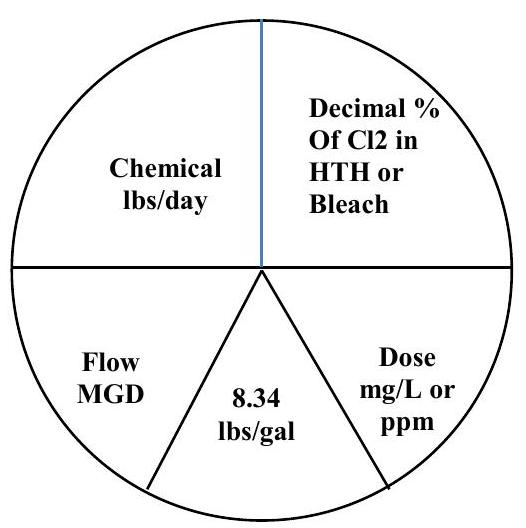
\includegraphics[max width=\textwidth]{2022_09_16_0c6b804a9b26a8df4e8fg-11}

Example:

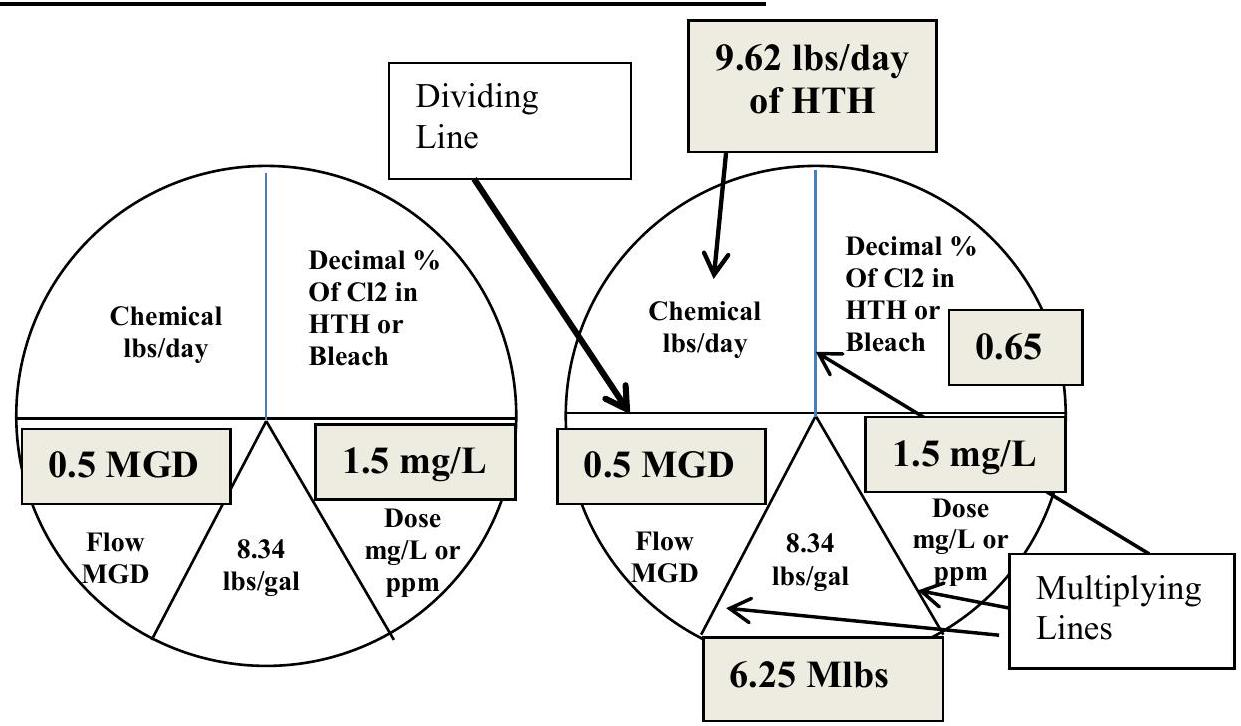
\includegraphics[max width=\textwidth]{2022_09_16_0c6b804a9b26a8df4e8fg-11(1)}

The well is pumping 0.5 MGD. You desire a dose of $1.5 \mathrm{mg} / \mathrm{L}$. How many lbs of $\mathrm{HTH}$ do you need to feed per day?

$1^{\text {st }}$ Place the numbers where they belong on the pie as shown above

You need to realize that the numbers on the bottom half of the pie represent $100 \%$ Chlorine Not $\mathrm{HTH}$ or any other percent of Chlorine such as bleach etc.

$\mathrm{HTH}$ is only $65 \%$ chlorine which in decimal form is $0.65$

$2^{\text {nd }}$ You need to multiply all the bottom numbers to find out how many lbs of $100 \%$ Chlorine you would need.

$0.5 \mathrm{MGD} \times 8.34 \mathrm{lbs} / \mathrm{gal} \times 1.5 \mathrm{mg} / \mathrm{L}=6.25 \mathrm{Mlbs}$ (again this is $100 \%$ chlorine)

Remember the way a pie works you need only remember that the half that needs no other information is divided by the half that is needing information to be full. In this case the bottom is full and the top needs information so the bottom number of $6.25 \mathrm{Mlbs}$ of Chlorine is divided by $0.65$.

\section{$6.25 \mathrm{Mlbs} \div 0.65=\mathbf{9 . 6 2} \mathrm{lbs} /$ day of $\mathbf{H T H}$}
Now work the same problem using the formula given to us to use by DEQ. However, you notice the formula given is only for $100 \%$ chlorine you have to add in the difference in $\%$.
$$
\text { Chemical Feed,lbs }=(\text { Dose, } m g / L x 8.34 \mathrm{lbs} / \mathrm{gal} x \text { Flow, } \mathrm{MGD})
$$
You have to rewrite this to look like the following
$$
\begin{gathered}
\text { Chemical Feed, } l b s=\frac{(\text { Dose }, m g / L \times 8.34 \mathrm{lbs} / \mathrm{gal} x \text { Flow, } M G D)}{0.65 \mathrm{HTH}} \\
\text { Chemical Feed, lbs }=\frac{(1.5 \text { Dose }, m g / L \times 8.34 \mathrm{lbs} / \mathrm{gal} x 0.5 \mathrm{Flow}, M G D)}{0.65 \mathrm{HTH}}
\end{gathered}
$$
Chemical Feed, lbs $=\mathbf{9 . 6 2} \mathbf{l b s} /$ day of $\mathbf{H T H}$

\section{Problems:}
\begin{enumerate}
  \setcounter{enumi}{38}
  \item The city water usage demand is $2.8 \mathrm{MGD}$ from the water plant. The water plant desire a dose of $2.5 \mathrm{mg} / \mathrm{L}$. How many lbs/day of $\mathrm{HTH}$ would you need to feed?

  \item The city water usage demand is $0.15 \mathrm{MGD}$ from the water plant. The water plant desire a dose of $1.5 \mathrm{mg} / \mathrm{L}$. How many $\mathrm{lbs} /$ day of $\mathrm{HTH}$ would you need to feed?\\

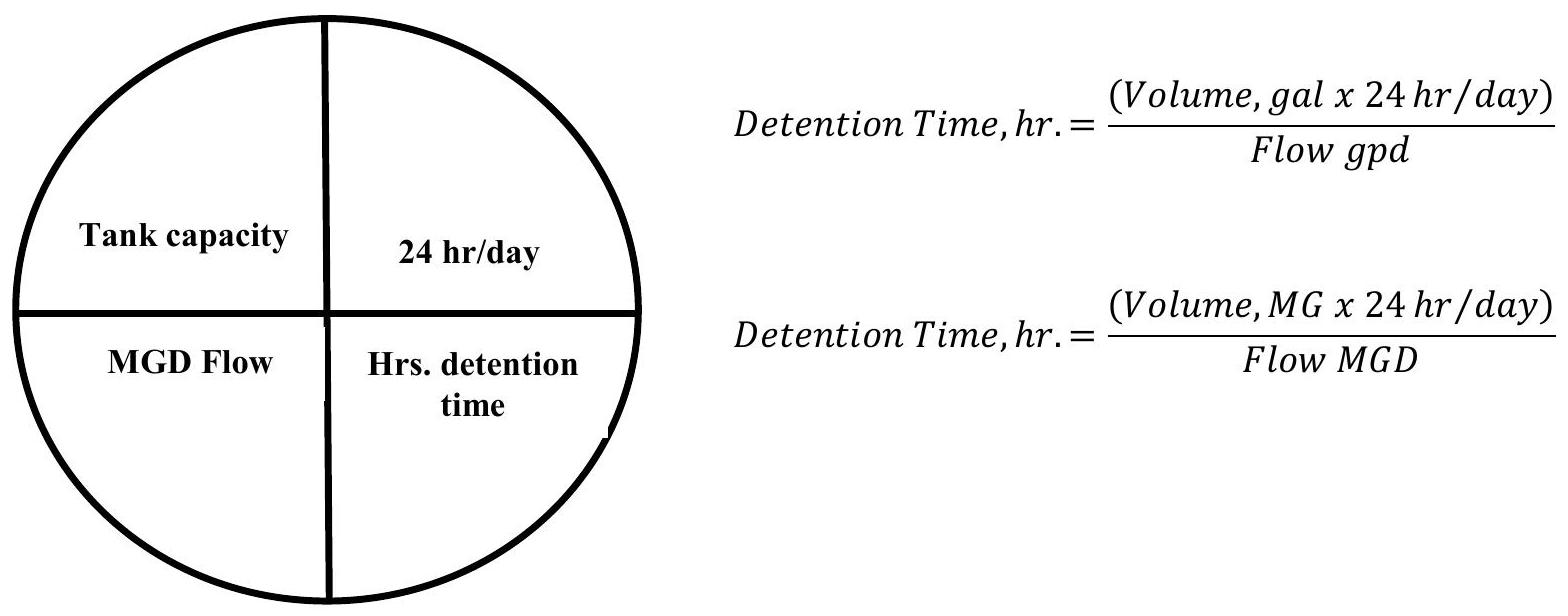
\includegraphics[max width=\textwidth]{2022_09_16_0c6b804a9b26a8df4e8fg-13}

\end{enumerate}
NOTE:

The pie on the DEQ handout sheet is formatted as MG \& MGD.

The formula sheet on the DEQ handout sheet is formatted as gallons. \& gpd.

It makes no difference if you use the $1^{\text {st }}$ or $2^{\text {nd }}$ format as long as you use the same format on the top of your equation or pie that you have on the bottom of the equation or pie.

Detention Time:\\

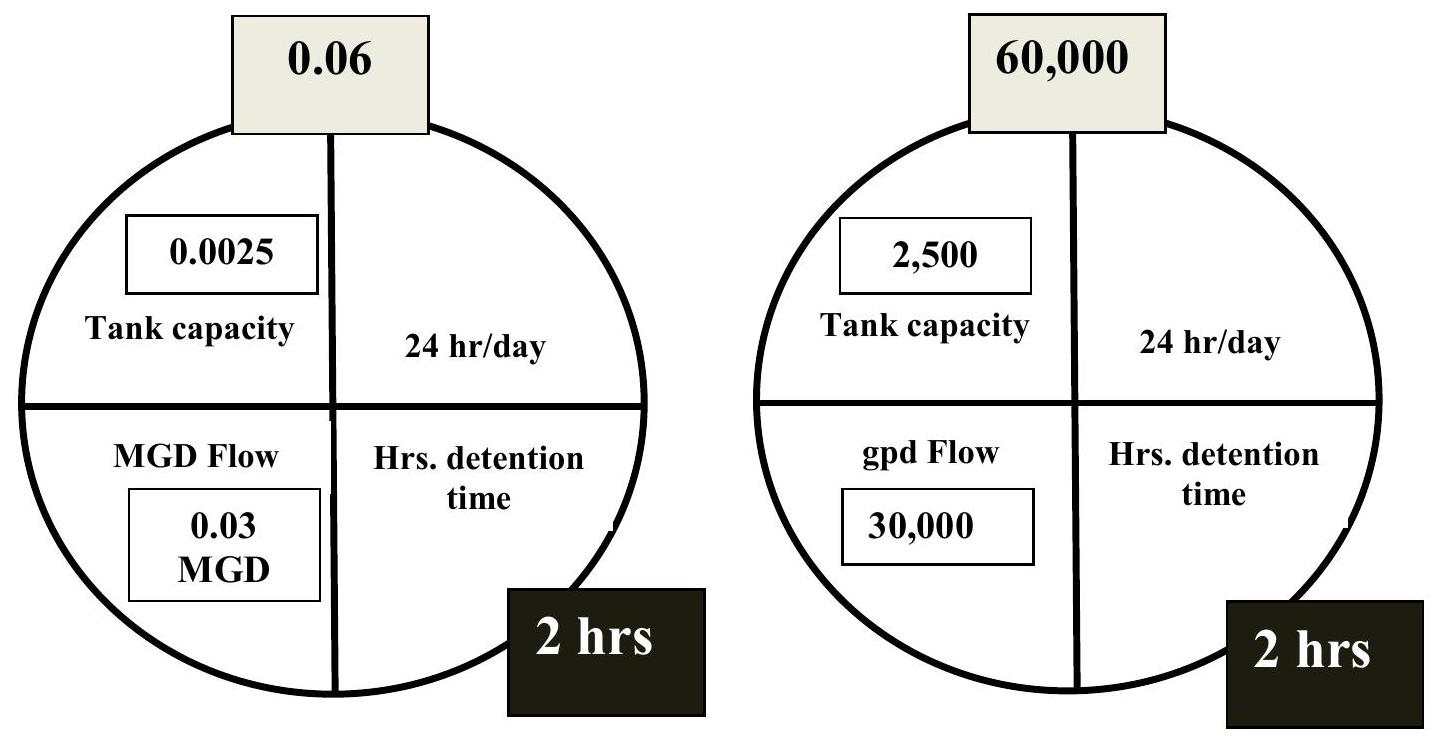
\includegraphics[max width=\textwidth]{2022_09_16_0c6b804a9b26a8df4e8fg-13(1)}

DEQ Formula:
$$
\begin{aligned}
&\text { Detention Time, } h r .=\frac{(\text { Volume, gal } x 24 \mathrm{hr} / \text { day })}{\text { Flow } g p d} \\
&\text { Detention Time, } h r .=\frac{(\text { Volume, } M G \times 24 \mathrm{hr} / \text { day })}{\text { Flow MGD }}
\end{aligned}
$$

\section{EXAMPLE:}
Determine the average detention time in hours for a basin that holds a volume of 2,500 gallons, that receives a flow of 30,000 gpd?\\
A. 2 hrs.\\
B. 4 hrs.\\
C. $20 \mathrm{hrs}$.\\
D. $9 \mathrm{hrs}$.

Detention Time, $h r .=\frac{(2,500 \text { Volume, gal } x 24 \mathrm{hr} / \text { day })}{30,000 \text { Flow gpd }}=2 \mathrm{hrs}$.

Detention Time, $h r .=\frac{(0.0025 \text { Volume, } M G x 24 h r / d a y)}{0.03 \text { Flow MGD }}=2 h r s$.

\section{Problems:}
\begin{enumerate}
  \setcounter{enumi}{40}
  \item What is the detention time in a storage tank 20 feet high and 30 feet in diameter when the rate of flow is $500,000 \mathrm{gal} /$ day?\\
A. $2.9$ hours\\
B. $5.1$ hours\\
C. $3.5$ hours
\end{enumerate}
Just as you learned earlier in this section on math the following formula will give you the ability to convert the dimensions given to volume in gallons.

$\left(\right.$ pi $\times \mathrm{r}^{2} \times$ depth $\left.\times 7.48 \mathrm{gal} / \mathrm{ft}^{3}\right)=$ volume in gallons

\begin{enumerate}
  \setcounter{enumi}{41}
  \item Basin $=38,000$ gal $\quad$ Flow $=65,000 \mathrm{gpd}$
\end{enumerate}
What is the detention time?\\
A. $1.4 \mathrm{hrs}$\\
B. $15 \mathrm{hrs}$\\
C. $14 \mathrm{hrs}$\\
D. $8 \mathrm{hrs}$

WEIR OVERFLOW:

\section{Circumference}
Circumference of a circle $=\pi \mathrm{x}$ diameter $\mathrm{ft}$.
$$
=3.14 \mathrm{x} \text { diameter } \mathrm{ft} \text {. }
$$
$$
\text { Weir Overflow } g p d / f t=\frac{\text { Flow } g p d}{\text { Weir Length ft. }}
$$

\section{EXAMPLE:}
The flow into a clarifier 80 foot diameter is $185 \mathrm{gpm}$. The weir is set back 1 foot. What is the weir overflow rate gpd/ft of weir?

Convert the information you have to fill in the information you need.

$1^{\text {st }}$ You were given 185 gpm but the formula is wanting gpd.

Simply convert to gpd: $\quad 185 \mathrm{gpm} \times 1440 \mathrm{~min} / \mathrm{day}=\mathbf{2 6 6 , 4 0 0} \mathbf{g p d}$ $2^{\text {nd }}$ You need to figure out the circumference of the weir.

Diameter is $80 \mathrm{ft}$. however the weir is set in $1 \mathrm{ft}$. on each side making the actual weir diameter $78 \mathrm{ft}$.

$3^{\text {rd }}$ Now that you know the diameter of the weir figure the circumference by using the circumference formula from below.

Circumference of a circle $=\pi \mathrm{x}$ diameter $\mathrm{ft}$.
$$
=3.14 \times 78
$$
$$
\begin{aligned}
& =244.92 \mathrm{ft} \text { of weir }
\end{aligned}
$$
Rounded to $=245 \mathrm{ft}$ of weir

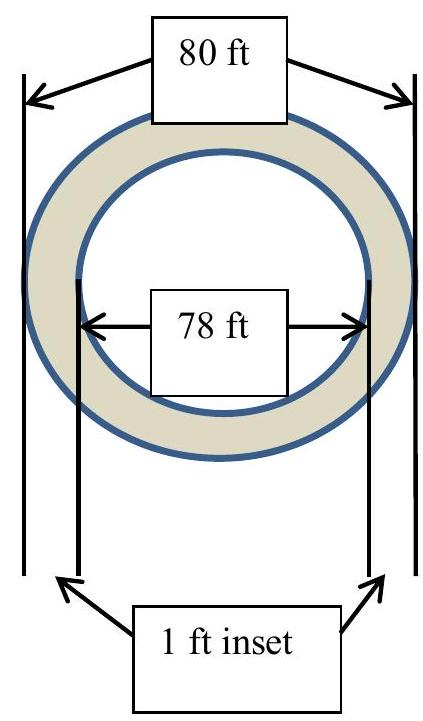
\includegraphics[max width=\textwidth]{2022_09_16_0c6b804a9b26a8df4e8fg-15}

Weir Overflow $g p d / f t=\frac{266,400 \text { Flow } g p d}{245 \text { Weir Length } f t .}=1,087 \mathrm{gpd} / \mathrm{ft}$ of weir

\section{Problems:}
\section{Weir Overflow $=1,087 g p d / f t$}
\begin{enumerate}
  \setcounter{enumi}{42}
  \item A tank with a weir set one foot in has an overall diameter of 35 feet and a flow of $0.22 \mathrm{MGD}$. What is the weir overflow rate in $\mathrm{gpd} / \mathrm{ft}$ of weir?\\
A. $2,189 \mathrm{gpd} / \mathrm{ft}$ of weir\\
B. $1,000 \mathrm{gpd} / \mathrm{ft}$ of weir\\
C. $228.6 \mathrm{gpd} / \mathrm{ft}$ of weir

  \item A clarifier with a weir set one foot in has an overall diameter of 32 feet and a flow of 1.1 MGD. What is the weir loading rate in gpm/foot of weir?\\
A. $9,553 \mathrm{gpd} /$ foot of weir\\
B. $897 \mathrm{gpd} /$ foot of weir\\
C. $11,677 \mathrm{gpd} / \mathrm{ft}$ of weir

\end{enumerate}
\section{SURFACE LOADING:}
$$
\text { Surface Loading } g p d / f t^{2}=\frac{\text { Flow } g p d}{\text { Surface Area ft }}
$$

\section{EXAMPLE:}
A primary clarifier has a diameter of 60 feet, the primary effluent flow is $2.3 \mathrm{MGD}$. What is the surface loading rate in $\mathrm{gpd} / \mathrm{ft}^{2}$ ?

Remember to convert MGD to gpd $2.3$ MGD x $1,000,000=$ Flow $\mathbf{2 , 3 0 0 , 0 0 0} \mathbf{g p d}$

How to figure surface area square feet example: $A=\pi r^{2}$
$$
\begin{aligned}
\text { Surface Area } &=3.14 \times \text { radius } \times \text { radius } \\
&=3.14 \times 30 \mathrm{ft} \times 30 \mathrm{ft} \\
&=\mathbf{2}, \mathbf{8 2 6} \mathbf{f t}^{2}
\end{aligned}
$$
Surface Loading gpd $/ f t^{2}=\frac{2,300,000 \text { Flow } g p d}{2,826 \text { Surface Area } f t^{2}}=\mathbf{8 1 3 . 8 7} \mathbf{g p d} / \mathbf{f t}^{2}$

\section{Problems:}
\begin{enumerate}
  \setcounter{enumi}{44}
  \item A circular clarifier has a diameter of 55 feet, the flow is $1.2$ MGD.
\end{enumerate}
What is the surface loading rate in $\mathrm{gpd} / \mathrm{ft}^{2}$ ?\\
A. $617.5 \mathrm{gpd} / \mathrm{ft}^{2}$\\
B. $505.3 \mathrm{gpd} / \mathrm{ft}^{2}$\\
C. $857.3 \mathrm{gpd} / \mathrm{ft}^{2}$

\begin{enumerate}
  \setcounter{enumi}{45}
  \item Calculate the surface loading rate on a clarifier $75 \mathrm{ft}$ in diameter with a flow rate of $4.1 \mathrm{MGD}$. What is the surface loading rate in $\mathrm{gpd} / \mathrm{ft}^{2}$ ?\\
A. $928 \mathrm{gpd} / \mathrm{ft}^{2}$\\
B. $1028 \mathrm{gpd} / \mathrm{ft}^{2}$\\
C. $1440 \mathrm{gpd} / \mathrm{ft}^{2}$

  \item Calculate the surface loading rate on a clarifier $40 \mathrm{ft}$ in diameter with a flow rate of $1.7 \mathrm{MGD}$. What is the surface loading rate in $\mathrm{gpd} / \mathrm{ft}^{2}$ ?\\
A. $818 \mathrm{gpd} / \mathrm{ft}^{2}$\\
B. $1128 \mathrm{gpd} / \mathrm{ft}^{2}$\\
C. $1354 \mathrm{gpd} / \mathrm{ft}^{2}$

\end{enumerate}
FILTRATION RATE:
$$
\text { Filtration Rate } g p m / f t^{2}=\frac{\text { Flow } g p m}{\text { Surface Area } f t^{2}}
$$

\section{Example:}
A flow rate of $0.5 \mathrm{MGD}$ is being filtered by a filter with the dimensions of $15 \mathrm{ft}$. wide and $20 \mathrm{ft}$. long. What is the filtration rate in $\mathrm{gpm} / \mathrm{ft}^{2}$ ?

$1^{\text {st }}$ Convert MGD to gpm $\quad 0.5$ MGD x $1,000,000=500,000$ gpd
$$
500,000 \mathrm{gpd} \div 1440 \mathrm{~min} / \text { day }=\mathbf{3 4 7} \mathbf{~ g p m}
$$
$2^{\text {nd }}$ Convert the dimensions to $\mathrm{ft}^{2} \quad 15 \mathrm{ft}$ wide $\times 20 \mathrm{ft}$ long $=\mathbf{3 0 0} \mathrm{ft}^{2}$
$$
\begin{aligned}
& \text { Filtration Rate } g p m / f t^{2}=\frac{347 \text { Flow } g p m}{300 \text { Surface Area } f t^{2}} \\
& \text { Filtration Rate }=1.16 \mathrm{gpm} / \mathrm{ft}^{2}
\end{aligned}
$$

\section{Problems:}
\begin{enumerate}
  \setcounter{enumi}{47}
  \item A flow rate of 600 gallons per minute is being filtered by 1200 square feet.
\end{enumerate}
What is the filter rate?\\
A. $2 \mathrm{gpm} / \mathrm{ft}^{2}$\\
B. $5.0 \mathrm{gpm} / \mathrm{ft}^{2}$\\
C. $.5 \mathrm{gpm} / \mathrm{ft}^{2}$

\begin{enumerate}
  \setcounter{enumi}{48}
  \item What is the filter rate in $\mathrm{gpm} / \mathrm{ft}^{2}$ with a Flow $=3 \mathrm{MGD} \quad$ Filter area $=1400 \mathrm{ft}^{2}$\\
A. $21.4 \mathrm{gpm} / \mathrm{ft}^{2}$\\
B. $1.5 \mathrm{gpm} / \mathrm{ft}^{2}$\\
C. . $15 \mathrm{gpm} / \mathrm{ft}^{2}$
\end{enumerate}
\section{Backwash rate:}
A backwash formula is not available in the DEQ handout however, it is a simple formula. The main thing to remember is the smaller of the two numbers will be divided by the larger of the two numbers.

The only two numbers you need to work this is the number of gallons that were filtered and the number of gallons you used to backwash with.

\section{Example:}
You have filtered 1.5 MG before needing to backwash. You used 35,000 gallons of water to backwash the filter. What is the backwash rate $\%$ ?

$1^{\text {st }}$ You will need to convert $\mathrm{MG}$ to gpd $1.5 \mathrm{MGx} 1,000,000=1,500,000 \mathrm{gpd}$

$2^{\text {nd }}$ Divide the smaller number by the larger number

$3^{\text {rd }}$ Your answer will be in decimal form so to convert it to $(\%)$ percent multiply by 100
$$
\text { Backwash rate } \%=\frac{\text { Gallons used to Backwash }}{\text { Gallons Filtered }}
$$
Backwash rate $\%=\frac{35,000 \mathrm{gal} .}{1,500,000 \mathrm{gpd}} \times 100$

Backwash rate $\%=0.023 \times 100$

\section{Backwash rate $=2.3 \%$}
\section{Problems:}
\begin{enumerate}
  \setcounter{enumi}{49}
  \item A filter is $30 \mathrm{ft}$ wide by $15 \mathrm{ft}$ long and flows 552,000 gallons before needing backwashed with $10,400 \mathrm{gal}$ and the backwash rate is $1.5 \mathrm{gpm} / \mathrm{ft}^{2}$. What is the percent of backwash?\\
A. $5.5 \%$\\
B. $3.5 \%$\\
C. $1.9 \%$
\end{enumerate}
California manual water treatment Plant Operation, Vol.1, Ch. 6, section 6.722, example 10

Equation:

Note: Always remember that the only two numbers you need for this problem is the gallons filtered and gallons used to backwash.

\begin{enumerate}
  \setcounter{enumi}{50}
  \item A filter has filtered $0.75 \mathrm{MG}$, you used 20,000 gallons to backwash.
\end{enumerate}
What is the percent of backwash?\\
A. $3.7 \%$\\
B. $2.7 \%$\\
C. $4.1 \%$ VELOCITY: $\quad$ Note: a number to remember $5,280 \mathrm{ft}$. $=1$ mile
$$
\text { Velocity, } f t / \min =\frac{\text { Distance }, f t .}{\text { Time }, \text { min. }}
$$
Example:

Water is traveling $1.5$ miles in $1.75$ hours. What is the velocity in $\mathrm{ft} / \mathrm{min}$ ?

$1^{\text {st }}$ Convert miles to ft. $\quad 1.5$ miles x $5,280 \mathrm{ft} / \mathrm{mile}=7,920 \mathrm{ft}$.

$2^{\text {nd }}$ Convert hours to $\min . \quad 1.75$ hrs. $\times 60 \mathrm{~min} / \mathrm{hr}$. $=105 \mathrm{~min} .$

$3^{\text {rd }}$ Fill in the formula and calculate
$$
\begin{aligned}
\text { Velocity, } f t / \min &=\frac{7,920 \text { Distance, } f t}{105 \text { Time }, \text { min }} \\
\text { Velocity } &=75.4 \mathrm{ft} / \min
\end{aligned}
$$
Problems:

\begin{enumerate}
  \setcounter{enumi}{51}
  \item Water is traveling 1 mile in $1.25$ hours. What is the velocity in feet per min.?\\
A. $70 \mathrm{ft} / \mathrm{min}$\\
B. $4224 \mathrm{ft} / \mathrm{min}$\\
C. $0.013 \mathrm{ft} / \mathrm{min}$

  \item Water is traveling $1450 \mathrm{ft}$ in $.5$ hours. What is the velocity in feet per min.?\\
A. $35 \mathrm{ft} / \mathrm{min}$\\
B. $48 \mathrm{ft} / \mathrm{min}$\\
C. $57 \mathrm{ft} / \mathrm{min}$

\end{enumerate}
Example of a more complex problem:

Water is flowing through a 10 "diameter pipe at a rate of 1,375 gpm.

What is the velocity of water in $\mathrm{ft} / \mathrm{sec}$ ?

$1^{\text {st }}$ How many gallons is in 1 foot of this pipe?

Formula $\left(\pi r^{2} \mathrm{ft}\right.$. x length $\mathrm{ft}$. $\left.\times 7.48 \mathrm{gal} / \mathrm{ft}^{3}\right)$

A. Figure Diameter in feet

$10 " \div 12 "=0.8333$ round to $0.83 \mathrm{ft}$. DIAMETER

B. Figure Radius

$0.83 \mathrm{ft}$. DIAMETER $\div 2=0.4166$ round to $0.42 \mathrm{ft}$. $\mathrm{RADIUS}$

C. $\left(3.14 \times 0.42 \mathrm{ft}\right.$. $\times 0.42 \mathrm{ft}$. x $1 \mathrm{ft}$. $\left.7.48 \mathrm{gal} / \mathrm{ft}^{3}\right)=4.143$ gal. round to $4.1$ gallons

$2^{\text {nd }}$ Figure how many $\mathrm{ft} / \mathrm{min} .$

$1,375 \mathrm{gpm} \div 4.1=335.3658 \mathrm{ft} / \mathrm{min}$ round to $335.4 \mathrm{ft} / \mathrm{min}$

$3^{\text {rd }}$ Reduce to $\mathrm{ft} / \mathrm{sec}$

$335.4 \mathrm{ft} / \mathrm{min} \div 60=5.5894 \mathrm{ft} / \mathrm{sec}$ round to $5.6 \mathbf{f t} / \mathbf{s e c}$

\section{Problems:}
\begin{enumerate}
  \setcounter{enumi}{53}
  \item Water is flowing through a $8 "$ diameter pipe at a rate of $1,850 \mathrm{gpm}$. What is the velocity of water in $\mathrm{ft} / \mathrm{sec}$ ?

  \item Water is flowing through a 18 "diameter pipe at a rate of $2,875 \mathrm{gpm}$. What is the velocity of water in $\mathrm{ft} / \mathrm{sec}$ ?

\end{enumerate}
\section{FLOW ft $3 /$ min:}
$$
\text { Flow, } f t^{3} / \min =\text { Area, } f t^{2} x \text { Velocity, } f t / \min
$$
This question is asking for $\mathrm{ft}^{3} / \mathrm{min}$. We know to get $\mathrm{ft}^{3}$ we need 3 foot measurements. Two (2) of the foot measurements come from the Surface Area of the pipe $\left(A=\pi r^{2}\right)$ The $3^{\text {rd }}$ foot measurement simply comes from the velocity $(\mathrm{ft} / \mathrm{min})$.

\section{Example:}
What is the flow in $\mathrm{ft} 3 / \mathrm{min}$ for a pipe that is 18 inches in diameter and the velocity is $150 \mathrm{ft} / \mathrm{min} . ?$

$1^{\text {st }}$ We need to find out the surface area of the pipe and to do that we need to convert some numbers to use the $\left(A=\pi r^{2}\right)$ formula.

The pipe is 18 inches in diameter, but we need ft. to make this work.

To do this we divide 18 inches by 12 inches/ft.
$$
\text { Diameter }=\frac{18 \text { inches }}{12 \text { inches } / \mathrm{ft}}=1.5 \mathrm{ft}
$$
NOTE: A common mistake here is to forget that you are still in Diameter when you need radius for the formula.
$$
\text { radius }=\frac{1.5 \mathrm{ft} .}{2}=0.75
$$
Now that we have the radius we can calculate the Surface area $\mathrm{ft}^{2}$.
$$
\begin{aligned}
&\text { Area } f t^{2}=3.14 \times .75 \times .75 \\
&\text { Area }=\mathbf{1 . 8 t ^ { 2 }}
\end{aligned}
$$
$2^{\text {nd }}$ If the Velocity is not in $\mathrm{ft} / \mathrm{min}$ convert until you get it there.

In this case the Velocity is already in $\mathrm{ft} / \mathrm{min}$ so we just need to fill in the formula and calculate. Velocity is $150 \mathrm{ft} / \mathrm{min}$.
$$
\begin{gathered}
\text { Flow, } f t^{3} / \mathrm{min}=\text { Area, } f t^{2} \times \text { Velocity, } f t / \mathrm{min} \\
\text { Flow, } f t^{3} / \mathrm{min}=1.8 \text { Area, } f t^{2} \times 150 \text { Velocity, } f t / \mathrm{min}
\end{gathered}
$$
$$
\text { Flow }=270 \mathrm{ft}^{3} / \mathrm{min} .
$$

\section{Problems:}
\begin{enumerate}
  \setcounter{enumi}{55}
  \item What is the flow in $\mathrm{ft} 3 / \mathrm{min}$ for a pipe that is 8 inches in diameter and the velocity is $100.8 \mathrm{ft} / \mathrm{min}$ ?\\
A. $25 \mathrm{ft}^{3} / \mathrm{min}$\\
B $35 \mathrm{ft}^{3} / \mathrm{min}$\\
C. $45 \mathrm{ft}^{3} / \mathrm{min}$

  \item What is the flow in $\mathrm{ft}^{3} / \mathrm{min}$ for a pipe that is 6 inches in diameter and the velocity is $225 \mathrm{ft} / \mathrm{min}$ ?\\
A. $22 \mathrm{ft} 3 / \mathrm{min}$\\
B $33 \mathrm{ft}^{3} / \min$\\
C. $44 \mathrm{ft}^{3} / \mathrm{min}$

\end{enumerate}
\section{Conversions:}
\section{Convert MGD to $\mathbf{f t}^{3} /$ sec}
To do this type of conversion you need convert the information given MGD to be in the format the answers are in. In this case $\mathrm{ft}^{3} / \mathrm{sec}$.

\section{Example:}
The water flow is $3.5 \mathrm{MGD}$. How many $\mathrm{ft}^{3} / \mathrm{sec}$ is the water traveling?

$1^{\text {st }}$ Convert MGD to gpd to $\mathrm{ft}^{3}$
$$
\text { 3.5 MGD x } 1,000,000=3,500,000 \mathrm{gpd} \div 7.48 \mathrm{gal} / \mathrm{ft}^{3}=467,914 \mathrm{ft}^{3} / \text { day }
$$
$2^{\text {nd }}$ Convert day to seconds

\section{Problems:}
$$
467,914 \mathrm{ft}^{3} / \text { day } \div 1440 \mathrm{~min} / \text { day } \div 60 \mathrm{sec} / \mathrm{min}=5.4 \mathbf{f t}^{3} / \mathbf{s e c}
$$

\begin{enumerate}
  \setcounter{enumi}{57}
  \item Convert 5.1 MGD to cubic feet per second.\\
A. $7.48 \mathrm{ft}^{3} / \mathrm{s}$\\
B. $1440 \mathrm{ft}^{3} / \mathrm{s}$\\
C. $7.9 \mathrm{ft}^{3} / \mathrm{s}$

  \item Convert 2.1 MGD to cubic feet per second.\\
A. $5.48 \mathrm{ft}^{3} / \mathrm{s}$\\
B. $3.25 \mathrm{ft}^{3} / \mathrm{s}$\\
C. $6.97 \mathrm{ft}^{3} / \mathrm{s}$

\end{enumerate}
\section{Convert $\mathbf{f t}^{3} /$ sec to gpm}
Here we are just reversing the process

\section{Example:}
Convert $4.7 \mathrm{ft}^{3} / \mathrm{sec}$ to gpm
$$
\begin{aligned}
&\mathrm{gpm}=4.7 \mathrm{ft}^{3} / \mathrm{sec} \times 7.48 \mathrm{gal} / \mathrm{ft}^{3} \times 60 \mathrm{sec} / \mathrm{min} \\
&\text { gpm }=\mathbf{2 , 1 0 9}
\end{aligned}
$$

\section{Problems:}
\begin{enumerate}
  \setcounter{enumi}{59}
  \item Convert $5.6 \mathrm{ft} 3 / \mathrm{s}$ to gallons per minute.\\
A. 3,700 gpm\\
B. $4,300 \mathrm{gpm}$\\
C. $2,500 \mathrm{gpm}$

  \item Convert $3.2 \mathrm{ft} 3 / \mathrm{s}$ to million gallons per day.\\
A. 3.2 MGD\\
B. $2.1 \mathrm{MGD}$\\
C. 4.7 MGD

\end{enumerate}
\section{HYDRAULIC SURFACE LOADINGRATE}
When figuring hydraulic surface loading rate you need to remember that the average wastewater production per person per day is 70 to 100 gallons. It is better when figuring loading rates to use the higher per person per day production. (100 gallons).

\section{Example:}
A discharging lagoon measures 125 feet wide and 450 feet long, it is serving a population of 400 people. What is the hydraulic surface loading rate in $\mathrm{gpd} / \mathrm{ft}^{2}$ ?

$\frac{(\text { Number of people } x 100 \text { gal per person per day) }}{(\text { length ft. } x \text { width } f \mathrm{f} .)}=$ Hydraulic surface loading rate in $g p d / f t^{2}$
$$
\begin{gathered}
\frac{(400 \text { people } x 100 \text { gallons per person })}{(450 \mathrm{ft} . \operatorname{long} x 125 \mathrm{ft} . \text { wide })}=\mathrm{gpd} / \mathrm{ft}^{2} \\
\frac{40,000 \mathrm{gallons}}{56,250 \mathrm{ft}^{2}}=0.71 \mathrm{gpd} / \mathrm{ft}^{2}
\end{gathered}
$$

\section{Problems:}
\begin{enumerate}
  \setcounter{enumi}{61}
  \item A discharging lagoon measures 100 feet wide and 250 feet long, it is serving a population of 250 people. What is the hydraulic surface loading rate in $\mathrm{gpd} / \mathrm{ft}^{2}$ ?

  \item A discharging lagoon measures 145 feet wide and 375 feet long, it is serving a population of 375 people. What is the hydraulic surface loading rate in $\mathrm{gpd} / \mathrm{ft}^{2}$ ?

\end{enumerate}
\section{ORGANIC LOADING RATE CALCULATIONS}
Organic loading rate calculations tell the operator the amount of food entering the plant. These calculations are used for wastewater treatment ponds, discharging lagoons, rotating biological contactors, or trickling filters.

\section{Example:}
There is a flow of $0.04$ MGD going to a discharging lagoon that measures 125 feet wide and 450 feet long with a BOD concentration is $125 \mathrm{mg} / \mathrm{L}$. What is the Organic loading rate $\mathrm{lbs} \mathrm{BOD} / \mathrm{ft}^{2}$ ?

Formula as written in DEQ handout
$$
\frac{B O D \text { applied,lbs }}{\text { Surface Area,ft }}=\text { Organic Loading, lbs. BOD/ft } 2
$$
Above formula explained on the following page. $\frac{(\text { Flow MGD } x \text { BOD mg/Lx 8.34lbs } / \text { gal })}{(\text { length ft. } x \text { width } f t .)}=$ Organic loading, lbs. $B O D / f^{2}$

$\frac{(\text { Flow } 0.04 \text { MGD } \times \text { BOD } 125 \mathrm{mg} / \mathrm{Lx} 8.34 \mathrm{lbs} / \mathrm{gal})}{(450 \mathrm{ft} \text {.long } \times 125 \mathrm{ft} \text {. wide })}=$ organic loading, lbs. BOD $/ \mathrm{ft}^{2}$
$$
\frac{41.7 \mathrm{lbs} B O D}{56,250 \mathrm{ft}^{2}}=\text { Organic loading, } 0.00074 \mathrm{lbs.} \mathrm{BOD} / \mathrm{ft}{ }^{2}
$$

\section{Problems:}
\begin{enumerate}
  \setcounter{enumi}{63}
  \item A flow of $0.1 \mathrm{MGD}$ with a BOD concentration of $108 \mathrm{mg} / \mathrm{L}$ is going to a discharge lagoon that measures $175 \mathrm{ft}$. wide and $500 \mathrm{ft}$. long. What is the Organic loading rate lbs $\mathrm{BOD} / \mathrm{ft}^{2} ?$

  \item A flow of $0.375 \mathrm{MGD}$ with a BOD concentration of $112 \mathrm{mg} / \mathrm{L}$ is going to a discharge lagoon that measures $125 \mathrm{ft}$. wide and $355 \mathrm{ft}$. long. What is the Organic loading rate $\mathrm{lbs}$ $\mathrm{BOD} / \mathrm{ft}^{2} ?$

\end{enumerate}
\section{Calculating lbs. of BOD/population}
\section{Example:}
A population of 233 will contribute about how many pounds of BOD per day?\\
A. $40 \mathrm{lbs} \mathrm{BOD}$\\
B. $50 \mathrm{lbs} \mathrm{BOD}$\\
C. $60 \mathrm{lbs} \mathrm{BOD}$

Approximately $0.17 \mathrm{lbs}$ of BOD $\quad(0.17)(233$ persons $)=39.61 \mathrm{lbs} / \mathrm{BOD}$

\section{Problems:}
\begin{enumerate}
  \setcounter{enumi}{65}
  \item A population of 26,650 will contribute about how many pounds of BOD per day?

  \item A population of 11,200 will contribute about how many pounds of BOD per day?

\end{enumerate}
\section{BOD loading lbs./day}
\section{Example}
Calculate the BOD loading lbs/day on a stream if the secondary effluent flow is $2.5$ MGD and BOD of secondary effluent is $20 \mathrm{mg} / \mathrm{L}$ :\\
A. $374 \mathrm{lbs} /$ day\\
B. $417 \mathrm{lbs} /$ day\\
C. $424 \mathrm{lbs} / \mathrm{day}$

You can use the same pie or formula that is used when figuring Dosage for any 100\% chemical (such as chlorine gas). Just change the wording.

Chemical Feed, lbs $=($ Dose, $\mathrm{mg} / \mathrm{L} x$ Flow, Mlbs $)$

BOD,$l b s /$ day $=($ Dose, $\mathrm{mg} / \mathrm{L} x$ Flow, Mlbs $)$ Formula expanded:
$$
\begin{gathered}
B O D, l b s / \text { day }=(\text { Dose }, m g / L x 8.34 l b s / g a l x \text { Flow, } M G D) \\
B O D, l b s / d a y=(20 \mathrm{mg} / L x 8.34 l b s / g a l \times 2.5 M G D) \\
B O D, l b s / d a y=417
\end{gathered}
$$

\section{Problems:}
\begin{enumerate}
  \setcounter{enumi}{67}
  \item Calculate the BOD loading lbs/day on a stream if the secondary effluent flow is $10 \mathrm{MGD}$ and BOD of secondary effluent is $17 \mathrm{mg} / \mathrm{L}$ :

  \item Calculate the BOD loading $\mathrm{lbs}$ /day on a stream if the secondary effluent flow is $21 \mathrm{MGD}$ and BOD of secondary effluent is $20 \mathrm{mg} / \mathrm{L}$ :

\end{enumerate}

\end{document}